\documentclass[parskip=full]{scrartcl}
\usepackage[utf8]{inputenc} % use utf8 file encoding for TeX sources
\usepackage[T1]{fontenc}    % avoid garbled Unicode text in pdf
\usepackage[german, english]{babel}  % german hyphenation, quotes, etc
\usepackage{graphicx}       % provides commands for including figures
\usepackage{rotating}
\usepackage{pdfpages}
\graphicspath{ {images/} }
\usepackage{hyperref}       % detailed hyperlink/pdf configuration
\hypersetup{                % ‘texdoc hyperref‘ for options
pdftitle={PSE : LAMeetsML},%
bookmarks=true,%
}
\usepackage{csquotes}       % provides \enquote{} macro for "quotes"
\usepackage[nonumberlist, acronym]{glossaries} % provides glossary commands
\usepackage{enumitem}
\usepackage{lscape}
\usepackage{caption}
\usepackage{placeins}


\makenoidxglossaries
%
%%Glossary
%

\newglossaryentry{algorithm}
{
	name=algorithm,
	plural=algorithms,
	description={In mathematics and computer science, an algorithm is an unambiguous specification of how to solve a class of problems. Algorithms can perform calculation, data processing and automated reasoning tasks}
}



\begin{document}

\begin{titlepage}
\centering
{\scshape\LARGE Karlsruher Institut für Technologie\par}
\vspace{1cm}
{\scshape\Large Design Document\par}
\vspace{1.5cm}
{\huge\bfseries Numerical Linear Algebra meets Machine Learning \par}
\vspace {2cm}

{\Large\itshape Fabian Koffer\par}
{\Large\itshape Simon Hanselmann\par}
{\Large\itshape Yannick Funk\par}
{\Large\itshape Dennis Leon Gr\"{o}tzinger\par}
{\Large\itshape Anna Katharina Ricker\par}

\vfill
Supervisors\par
Hartwig Anzt
Makus G\"{o}tz

\vfill
{\large\today\par}
\end{titlepage}

\tableofcontents
\newpage


\section{Class descriptions}

\subsection{Collector}
\subsection{Labeling Module}
\subsection{Training Moulde}
\subsubsection{Class Configuration File}
The configuration file is a text file. It is used to specify all necessary information the class neural network needs to train the neural network.If the user does not change anything in the configuration file, defaut options will be used.The configuration file is organized in four main categories. 
\begin{enumerate}
\item loading path of the set of matrices
\item saving path for the neural network
\item loading path for the neural network
\item model definition and hyperparameters
\end{enumerate}
\subsubsection{Class Neural Network}

\subsection{Classifier}
\subsection{Command line interface}
\subsection{Classes needed in more than one module}
\subsubsection{Class Matrix}


\section{Activity diagrams}


\subsection{Collector}
\subsection{Labeling Module}
\subsection{Training Moulde}
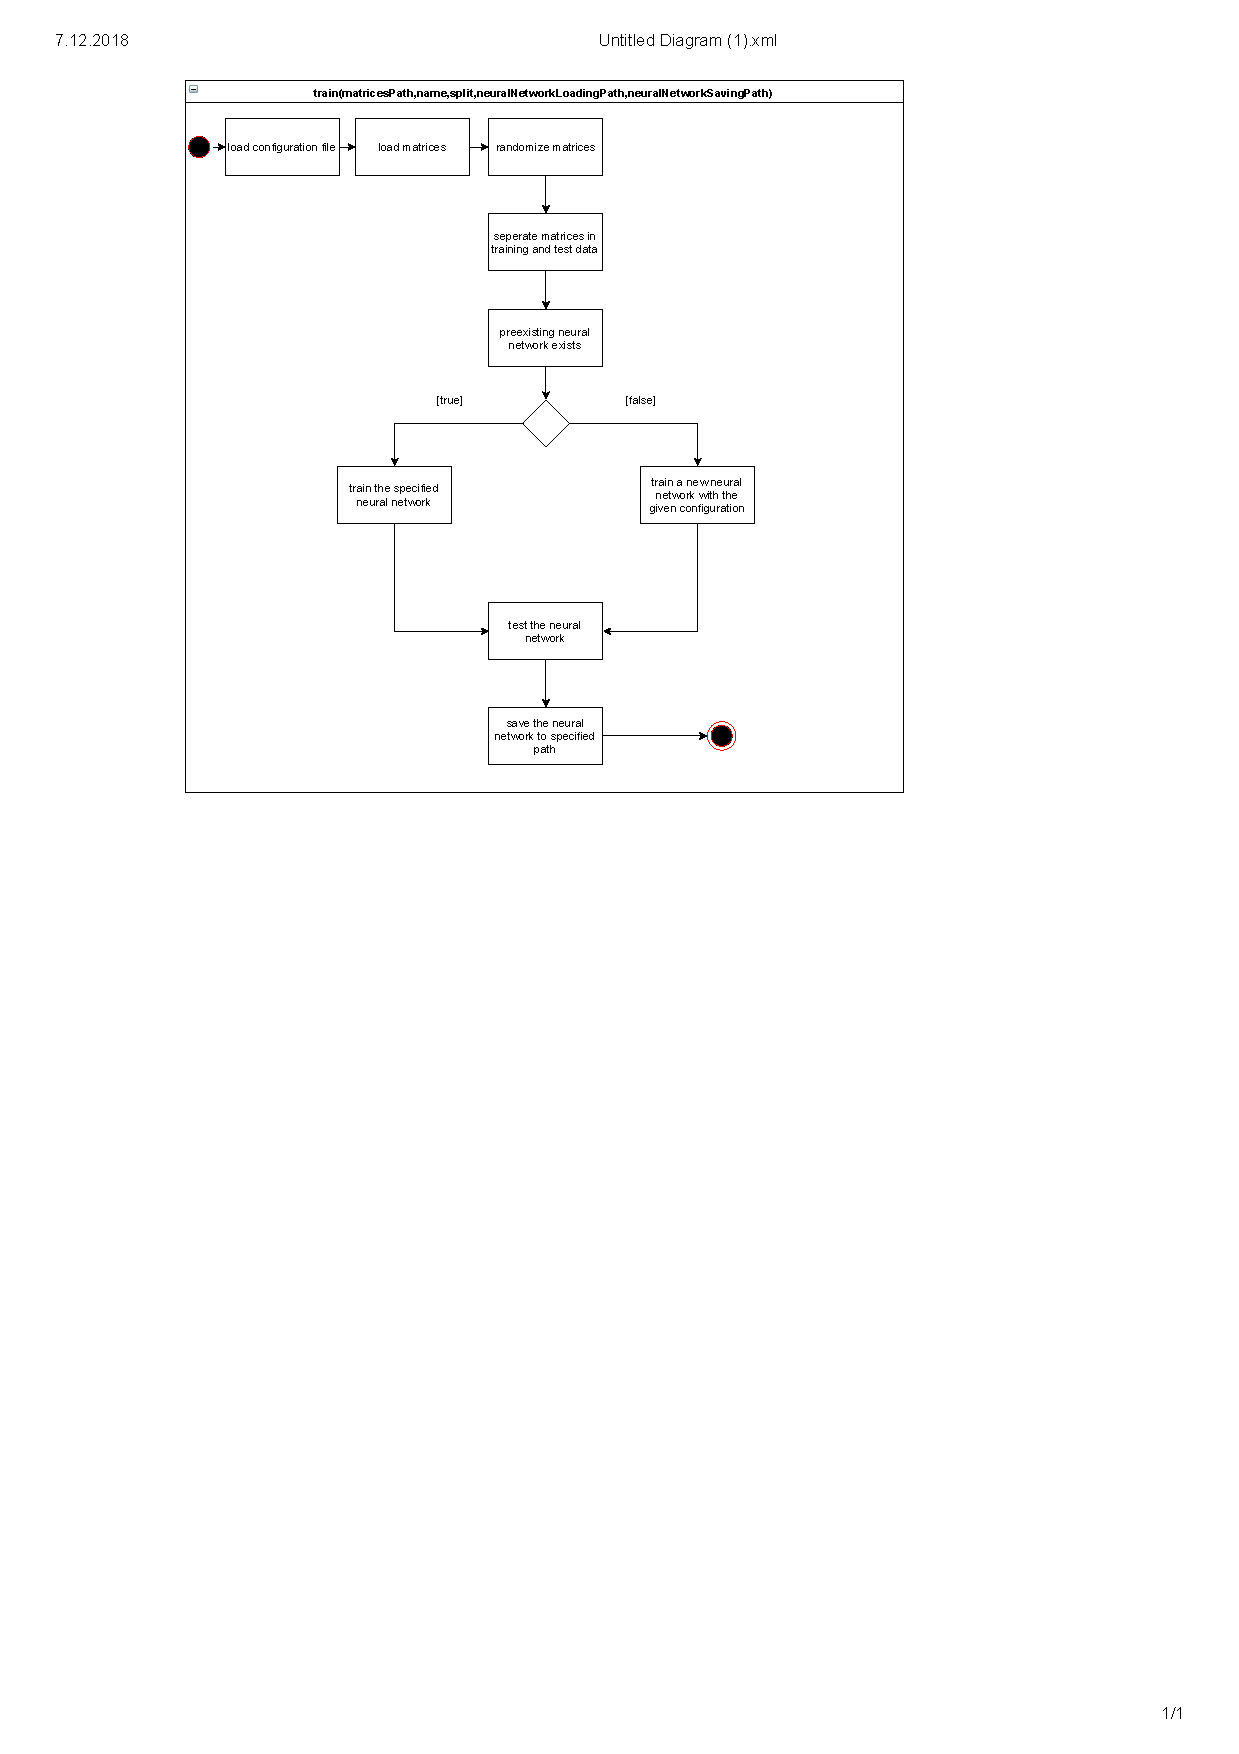
\includepdf[pages={1}]{ActivityDiagrams/TrainingModule}
\subsection{Classifier}

\section{Class diagrams}


\section{Sequence diagrams}

\section{Glossary}
%\glspl{collector}, labeling modle, neural network, classifier, default settings  \glspl{Dateiformat}

% % Automatisch generiertes Glossar (Latex zwei mal ausführen um Glossar anzuzeigen)
%
%\glsaddall % das sorgt dafür, dass alles Glossareinträge gedruckt werden, nicht nur die verwendeten. Das sollte nicht nötig sein!
\printnoidxglossaries

\end{document}
